\section{Benchmark NIST-5 "Battery"}
\label{sec:bench-5}

This is a heat conduction problem in a nonhomogeneous material.
It comes with an anisotropic solution with strong internal disruption
layers and singularities.
The solution has multiple point singularities in the interior at which
more than three different materials meet. These singularities are stronger than those
corresponding to reentrant corners \cite{demkowicz-1}.
The equation solved is given by

\begin{equation} \label{heat-conduction}
-\frac{\partial }{\partial x}\left(p(x, y)\frac{\partial u}{\partial x}\right)
-\frac{\partial }{\partial y}\left(q(x, y)\frac{\partial u}{\partial y}\right) = f
\end{equation}
in the domain $\Omega = (0, 8.4) \times (0, 24)$. Boundary conditions are zero Neumann on left edge, Newton on the rest of the boundary.
The right-hand side $f$ are constant functions (different in respective materials).
The solution of NIST-5 is shown in Fig. \ref{fig:sln-nist05}.

\begin{figure}[!ht]
\centering
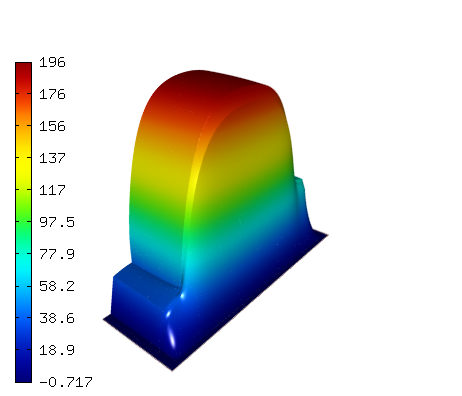
\includegraphics[height=5cm]{nist/nist-5/solution.png}
\caption{The solution to NIST-5 benchmark problem.}
\label{fig:sln-nist05}
\end{figure}

%\begin{figure}[!ht]
%\centering
%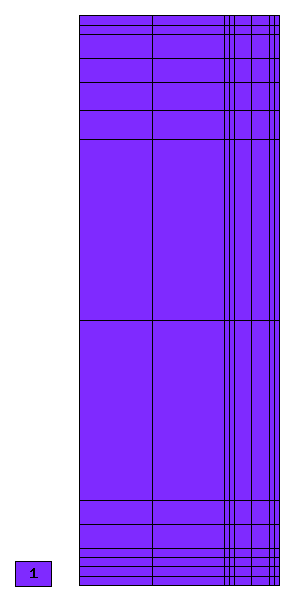
\includegraphics[height=5cm]{nist/nist-5/mesh_hp_aniso_init.png}\ \
%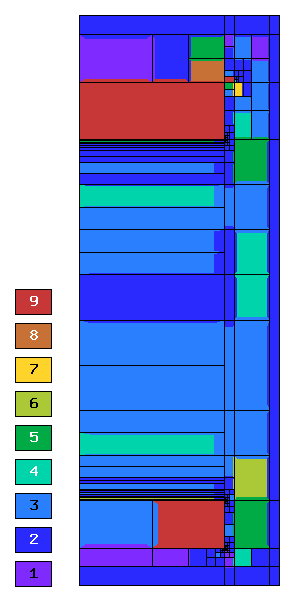
\includegraphics[height=5cm]{nist/nist-5/mesh_hp_aniso.png}
%\caption{Initial mesh (left) and final mesh (right) with 7450 DOF and the resulting relative error estimate in $H^1$-norm of 1.46775e-02 \% for $hp$-FEM with anisotropic refinements.}
%\label{fig:nist-5-hp-aniso}
%\end{figure}

%\begin{figure}[!ht]
%\centering
%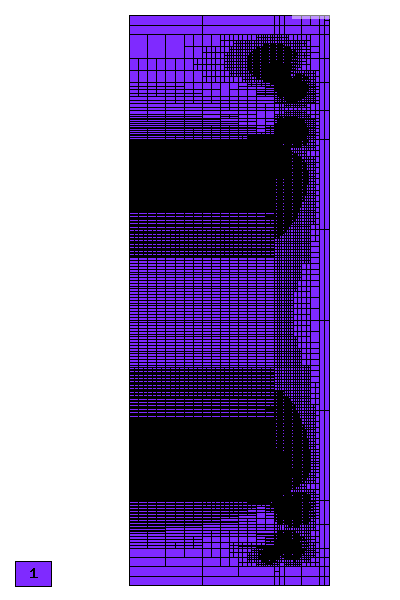
\includegraphics[height=5cm]{nist/nist-5/mesh_h1_aniso.png}\ \
%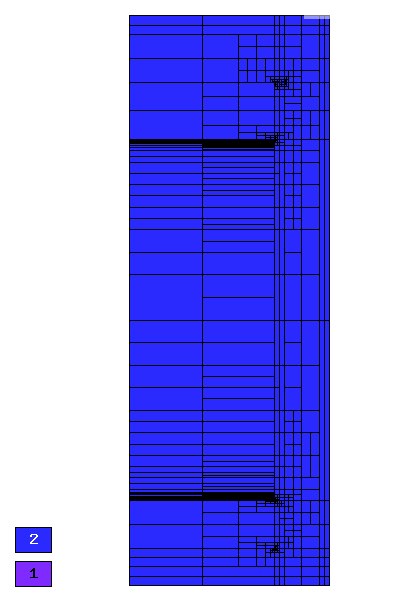
\includegraphics[height=5cm]{nist/nist-5/mesh_h2_aniso.png}
%\caption{Final mesh for $h$-FEM with linear and quadratic elements.}
%\label{fig:nist-5-h-aniso}
%\end{figure}

\begin{figure}[!ht]
\centering
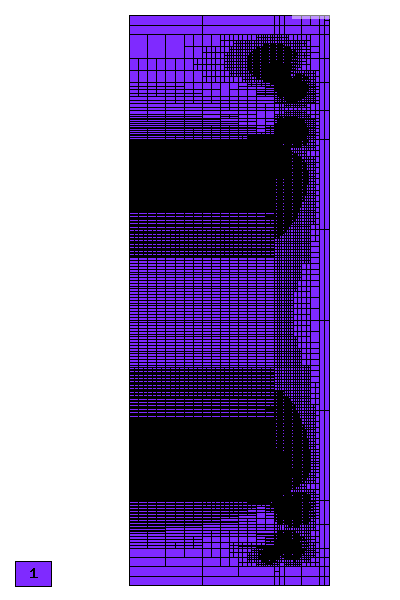
\includegraphics[height=5cm]{nist/nist-5/mesh_h1_aniso.png}
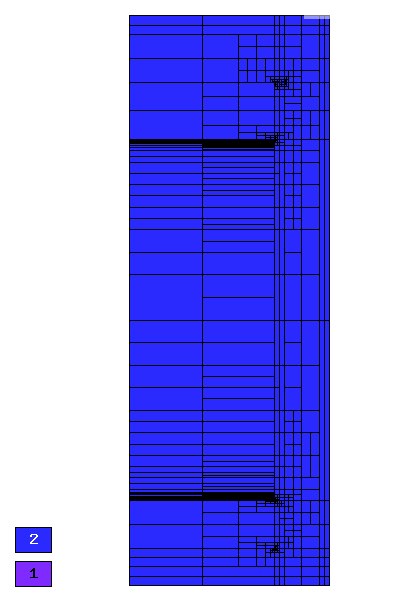
\includegraphics[height=5cm]{nist/nist-5/mesh_h2_aniso.png}
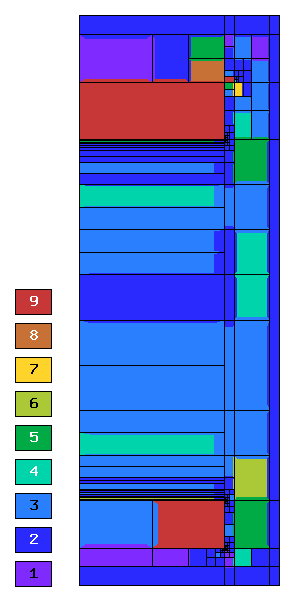
\includegraphics[height=5cm]{nist/nist-5/mesh_hp_aniso.png}
\caption{
Final mesh (left) with 55577 DOF and the resulting
relative error estimate in $H^1$-norm of 9.57345e-02 \% for $h$-FEM with linear elements.
Final mesh (middle) with 12483 DOF and the resulting
relative error estimate in $H^1$-norm of 1.34925e-02 \% for $h$-FEM with quadratic elements.
Final mesh (right) with 7450 DOF and the resulting 
relative error estimate in $H^1$-norm of 1.46775e-02 \% for $hp$-FEM with anisotropic refinements.}
\label{fig:nist-5-hp-aniso}
\end{figure}

Figs. \ref{fig:nist-5-conv} compare all
three approaches to automatic adaptivity from the point
of view of DOF and CPU convergence.

\begin{figure}[!ht]
\centering
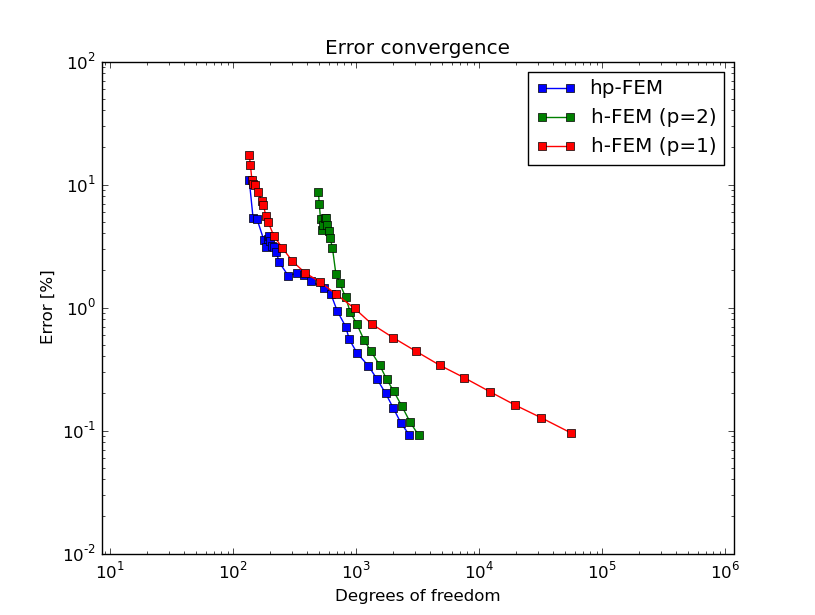
\includegraphics[height=5cm]{nist/nist-5/conv_dof_aniso.png}\ \
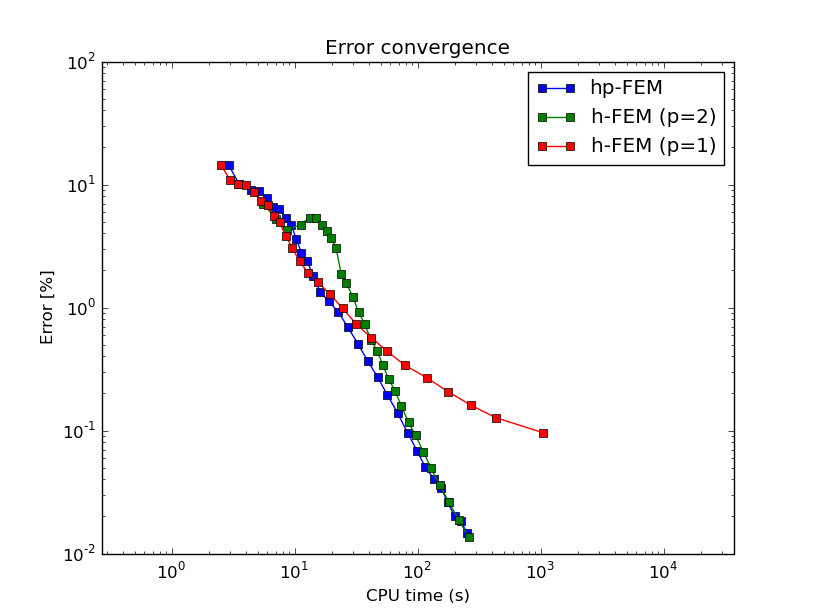
\includegraphics[height=5cm]{nist/nist-5/conv_cpu_aniso.png}
\caption{DOF and CPU time convergence graphs.}
\label{fig:nist-5-conv}
\end{figure}

